\documentclass[conference]{IEEEtran} % Use IEEE template in two-column format

% Required packages
\usepackage{graphicx} % For including images
\usepackage{amsmath, amssymb} % For mathematical symbols
\usepackage{cite} % For citations
\usepackage{hyperref} % For hyperlinks
\usepackage{listings} % For code formatting
\usepackage{float} % Images were moving added this package to address that

\lstset{
    basicstyle=\ttfamily\small, % Monospace font, small size
    breaklines=true,             % Enable automatic line breaking
    breakatwhitespace=false,     % Allow breaks anywhere
    columns=fullflexible,        % Better spacing for long lines
}


\begin{document}

\title{Assignment 1}

\author{
    \IEEEauthorblockN{Logan Bowles} \\
    \IEEEauthorblockA{University of North Carolina at Greensboro \\ Email: lbbowles2@uncg.edu}
}

\maketitle

\begin{abstract}
This is the paper for Assignment 1 and 2.  Designed to follow the requests of the Assignment1.pdf.
\end{abstract}

\section{Setting up the Programming Environment}

This section includes the uploaded screenshots of the Python environment and accompanying add-ons for it to run effectively. When it comes to my setup of the project, I didn’t really have to do anything because I have previously dropped this class and therefore already set up the environment.

That being said, the command below was the only one I believe I had to run last time to download OpenCV:

\begin{lstlisting}
/bin/bash -c "$(curl -fsSL https://raw.githubusercontent.com/Homebrew/install/HEAD/install.sh)"
\end{lstlisting}

Additionally, I had to install pandas by running the following command in Terminal while the environment was open:

\begin{lstlisting}
python3 -m pip install pandas
\end{lstlisting}

Everything else was straightforward after downloading Anaconda and installing the required packages through it.

The screenshots of the Environment and tools for the Environment setup are provided as Figures \ref{fig:task1_1}-\ref{fig:task1_2}.

\begin{figure}[H]
    \centering
    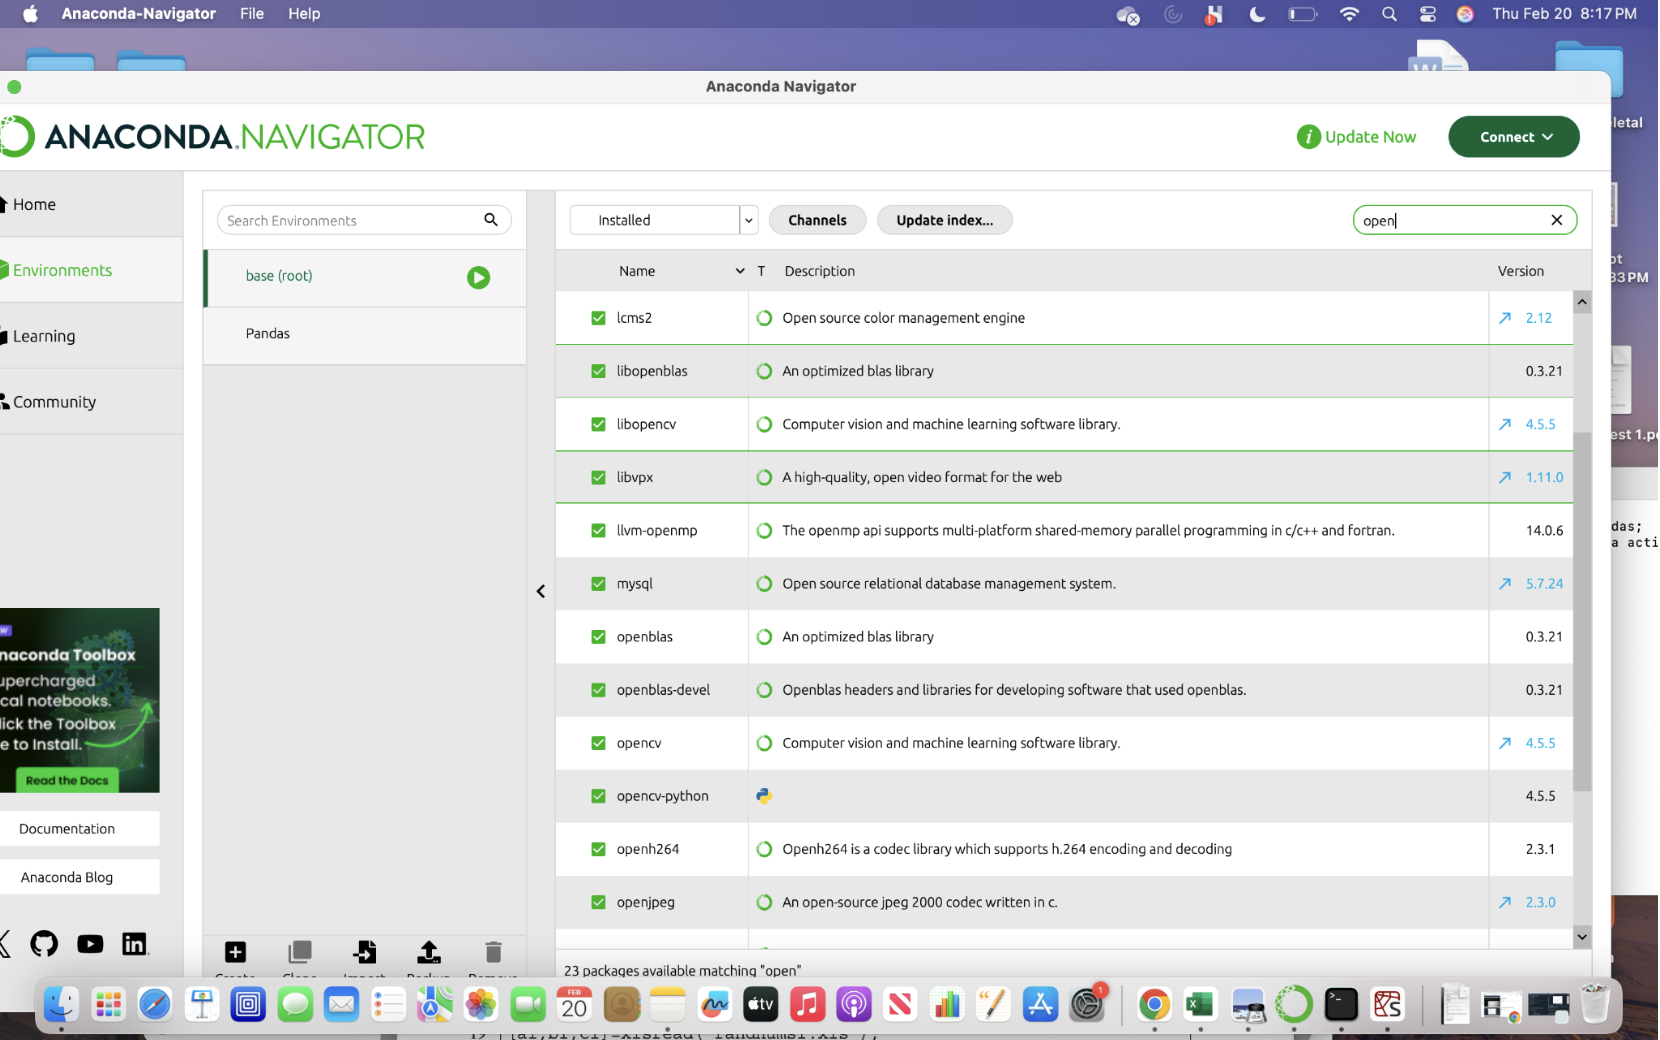
\includegraphics[width=0.5\linewidth]{task1_1.png}
    \caption{Screenshot of Anaconda and packages for Environment}
    \label{fig:task1_1}
\end{figure}

\begin{figure}[H]
    \centering
    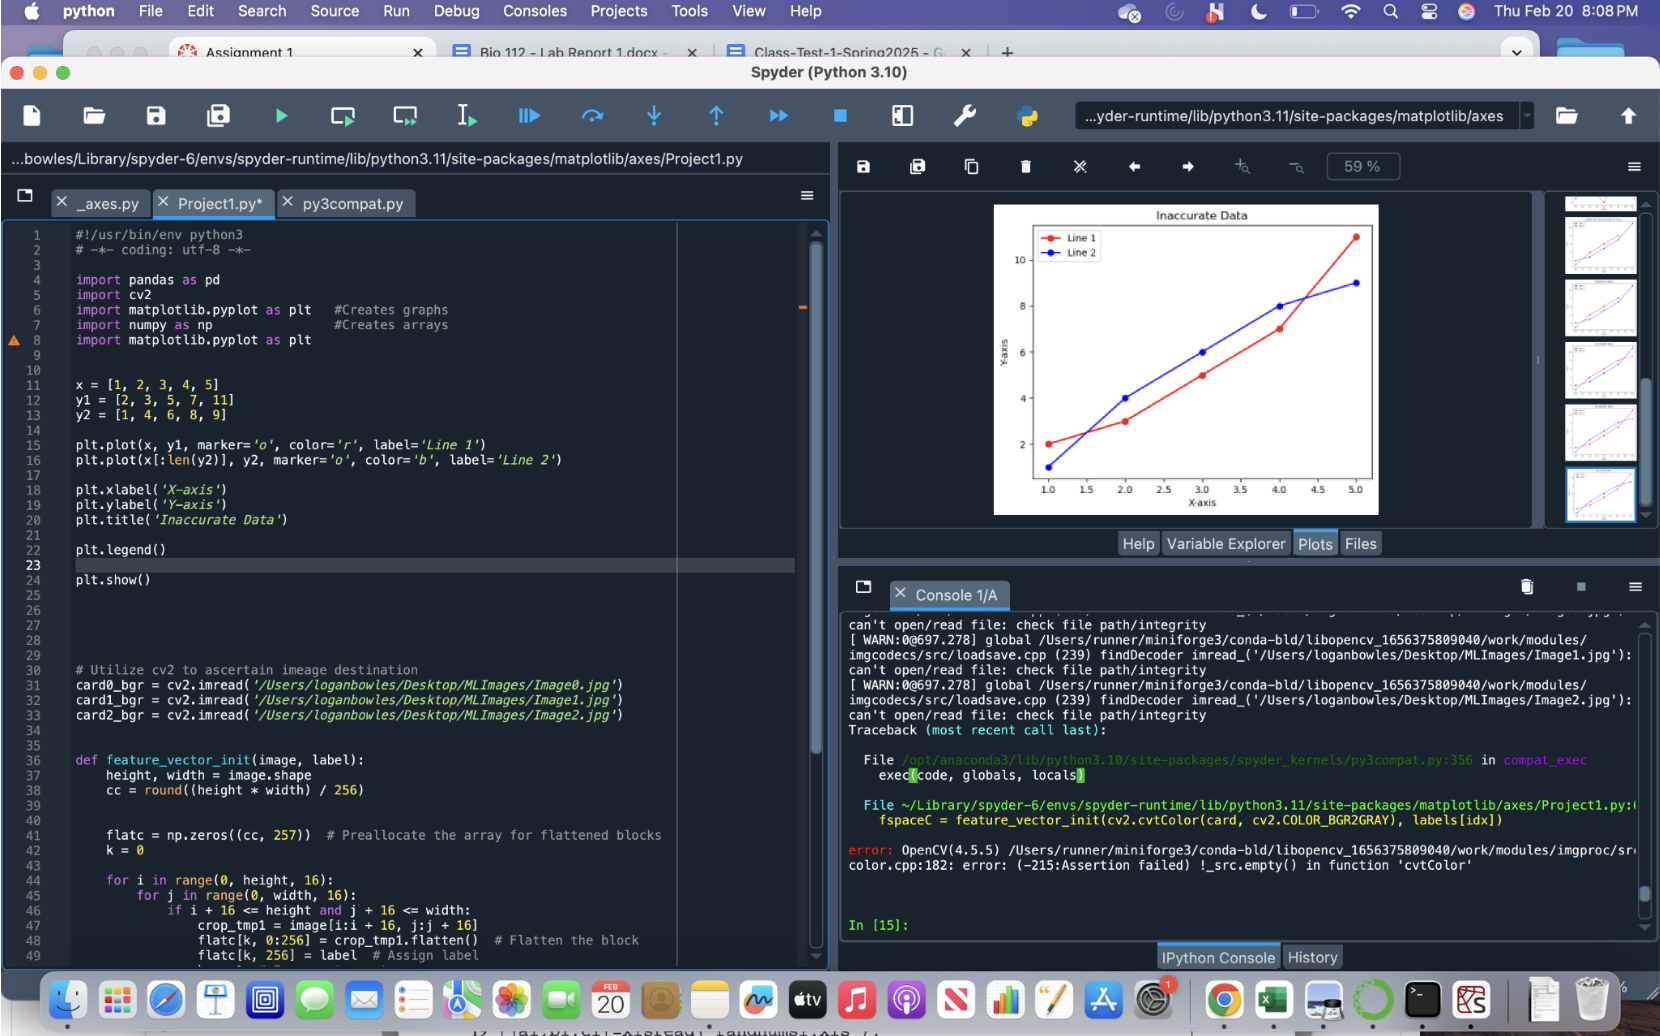
\includegraphics[width=0.5\linewidth]{task1_2.png}
    \caption{Screenshot of Environment open}
    \label{fig:task1_2}
\end{figure}


\section{Ascertaining Data Sets}

Just as was recommended in the Assignment1.pdf, I have named the images I will be utilizing as 'image0', 'image1', and 'image2'. I have chosen:
\begin{itemize}
    \item *image0* - '2.jpg' under the 'apples' folder.
    \item *image1* - '52.jpg' in the 'grapes' folder.
    \item *image2* - '25.jpg' in the 'lemons' folder.
\end{itemize}

All of these images are part of the FIDS30 dataset \cite{Skrjanec2013}. 

I chose these specific fruits to ensure they all have distinct primary colors, making classification easier for the machine learning model. I also ensured that the images I selected had minimal background interference, allowing me to avoid annoying modifications such as  cropping.

Figures \ref{fig:image0}-\ref{fig:screenshot2} display the selected images and folder structure.

\begin{figure}[H]
    \centering
    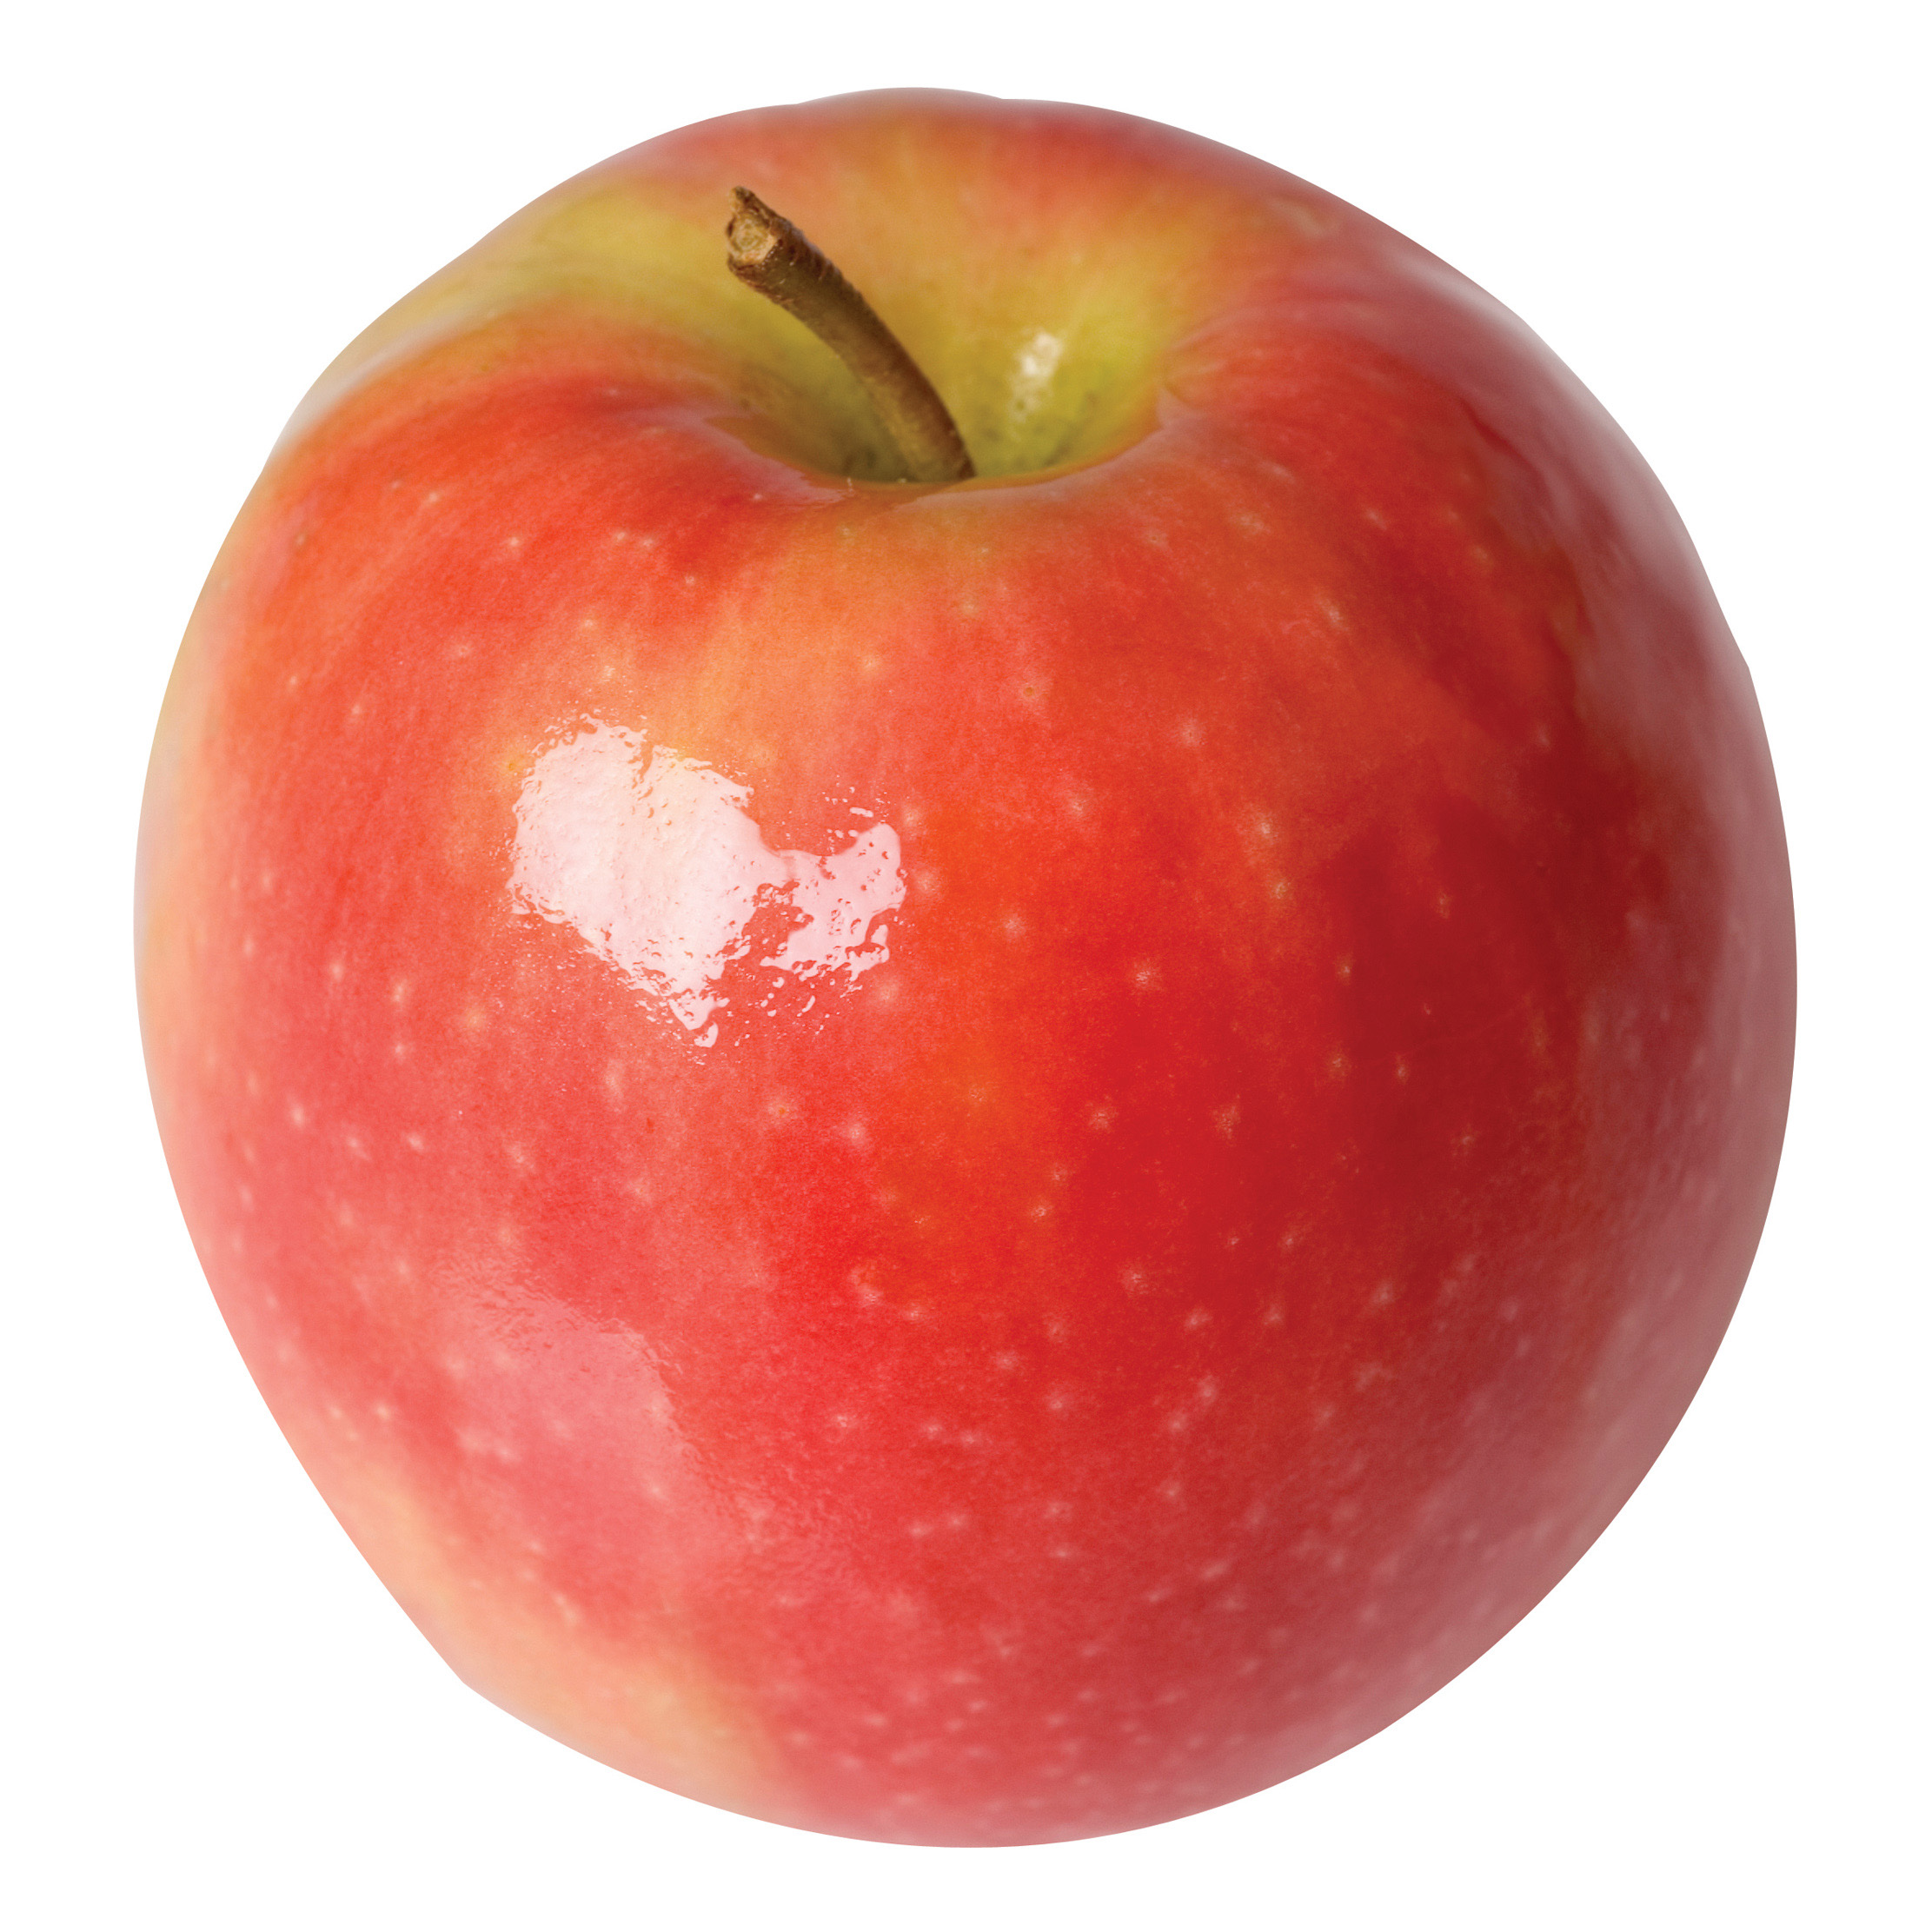
\includegraphics[width=0.5\linewidth]{image0.jpg}
    \caption{Apple sample - image0.jpg}
    \label{fig:image0}
\end{figure}

\begin{figure}[H]
    \centering
    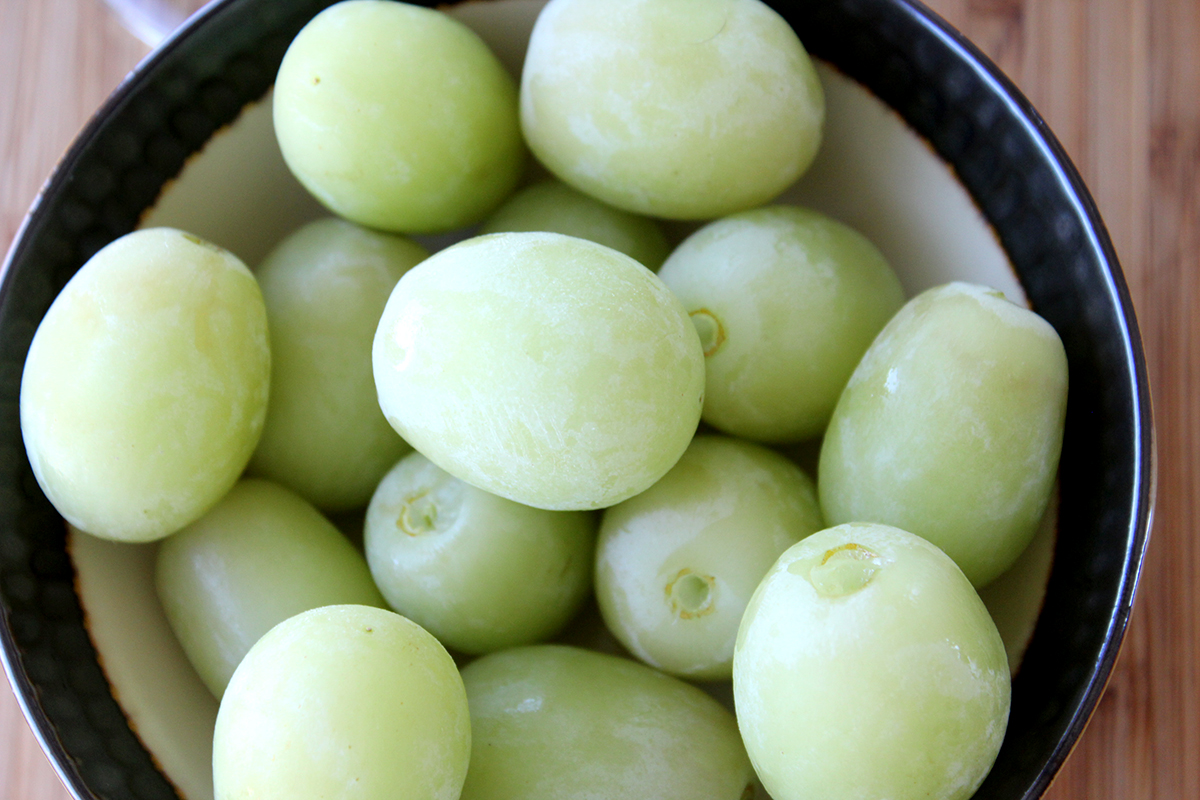
\includegraphics[width=0.5\linewidth]{image1.jpg}
    \caption{Grape sample - image1.jpg}
    \label{fig:image1}
\end{figure}

\begin{figure}[H]
    \centering
    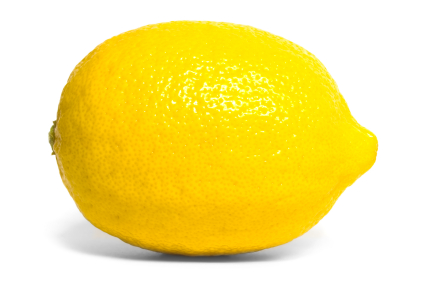
\includegraphics[width=0.5\linewidth]{image2.jpg}
    \caption{Lemon sample - image2.jpg}
    \label{fig:image2}
\end{figure}

\begin{figure}[H]
    \centering
    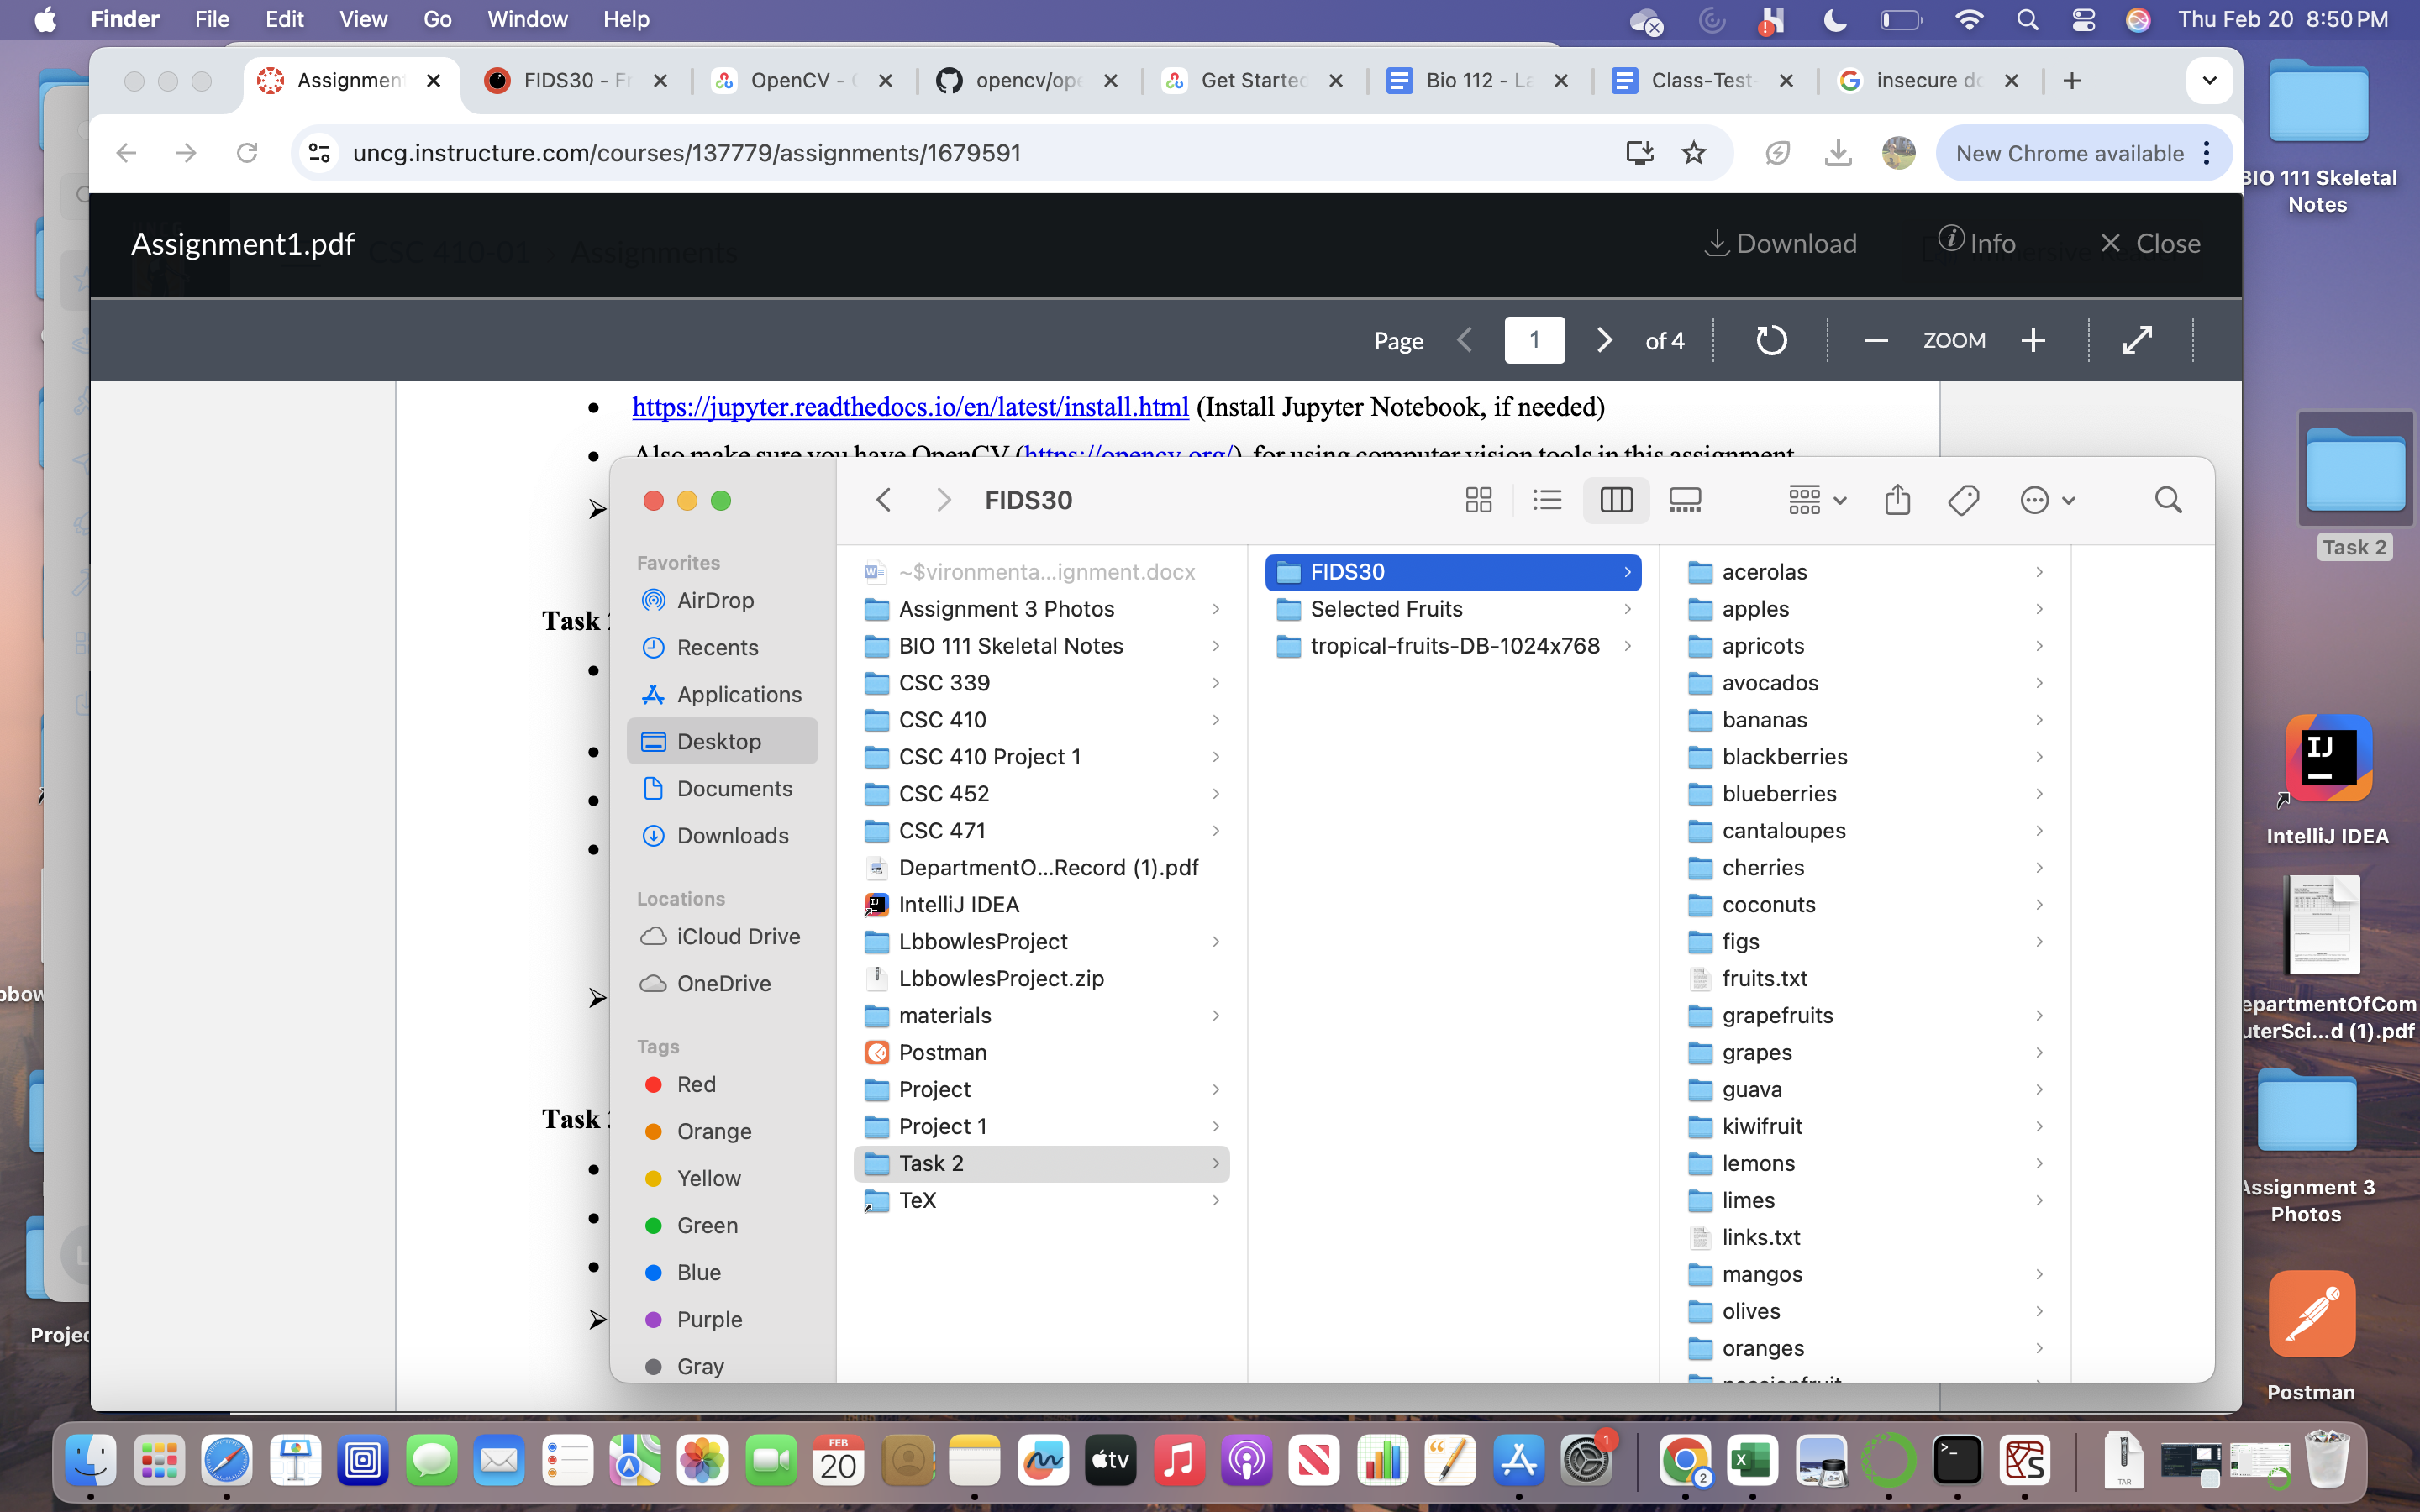
\includegraphics[width=0.5\linewidth]{datafolder.png}
    \caption{Screenshot of FIDS30 folder}
    \label{fig:screenshot1}
\end{figure}

\begin{figure}[H]
    \centering
    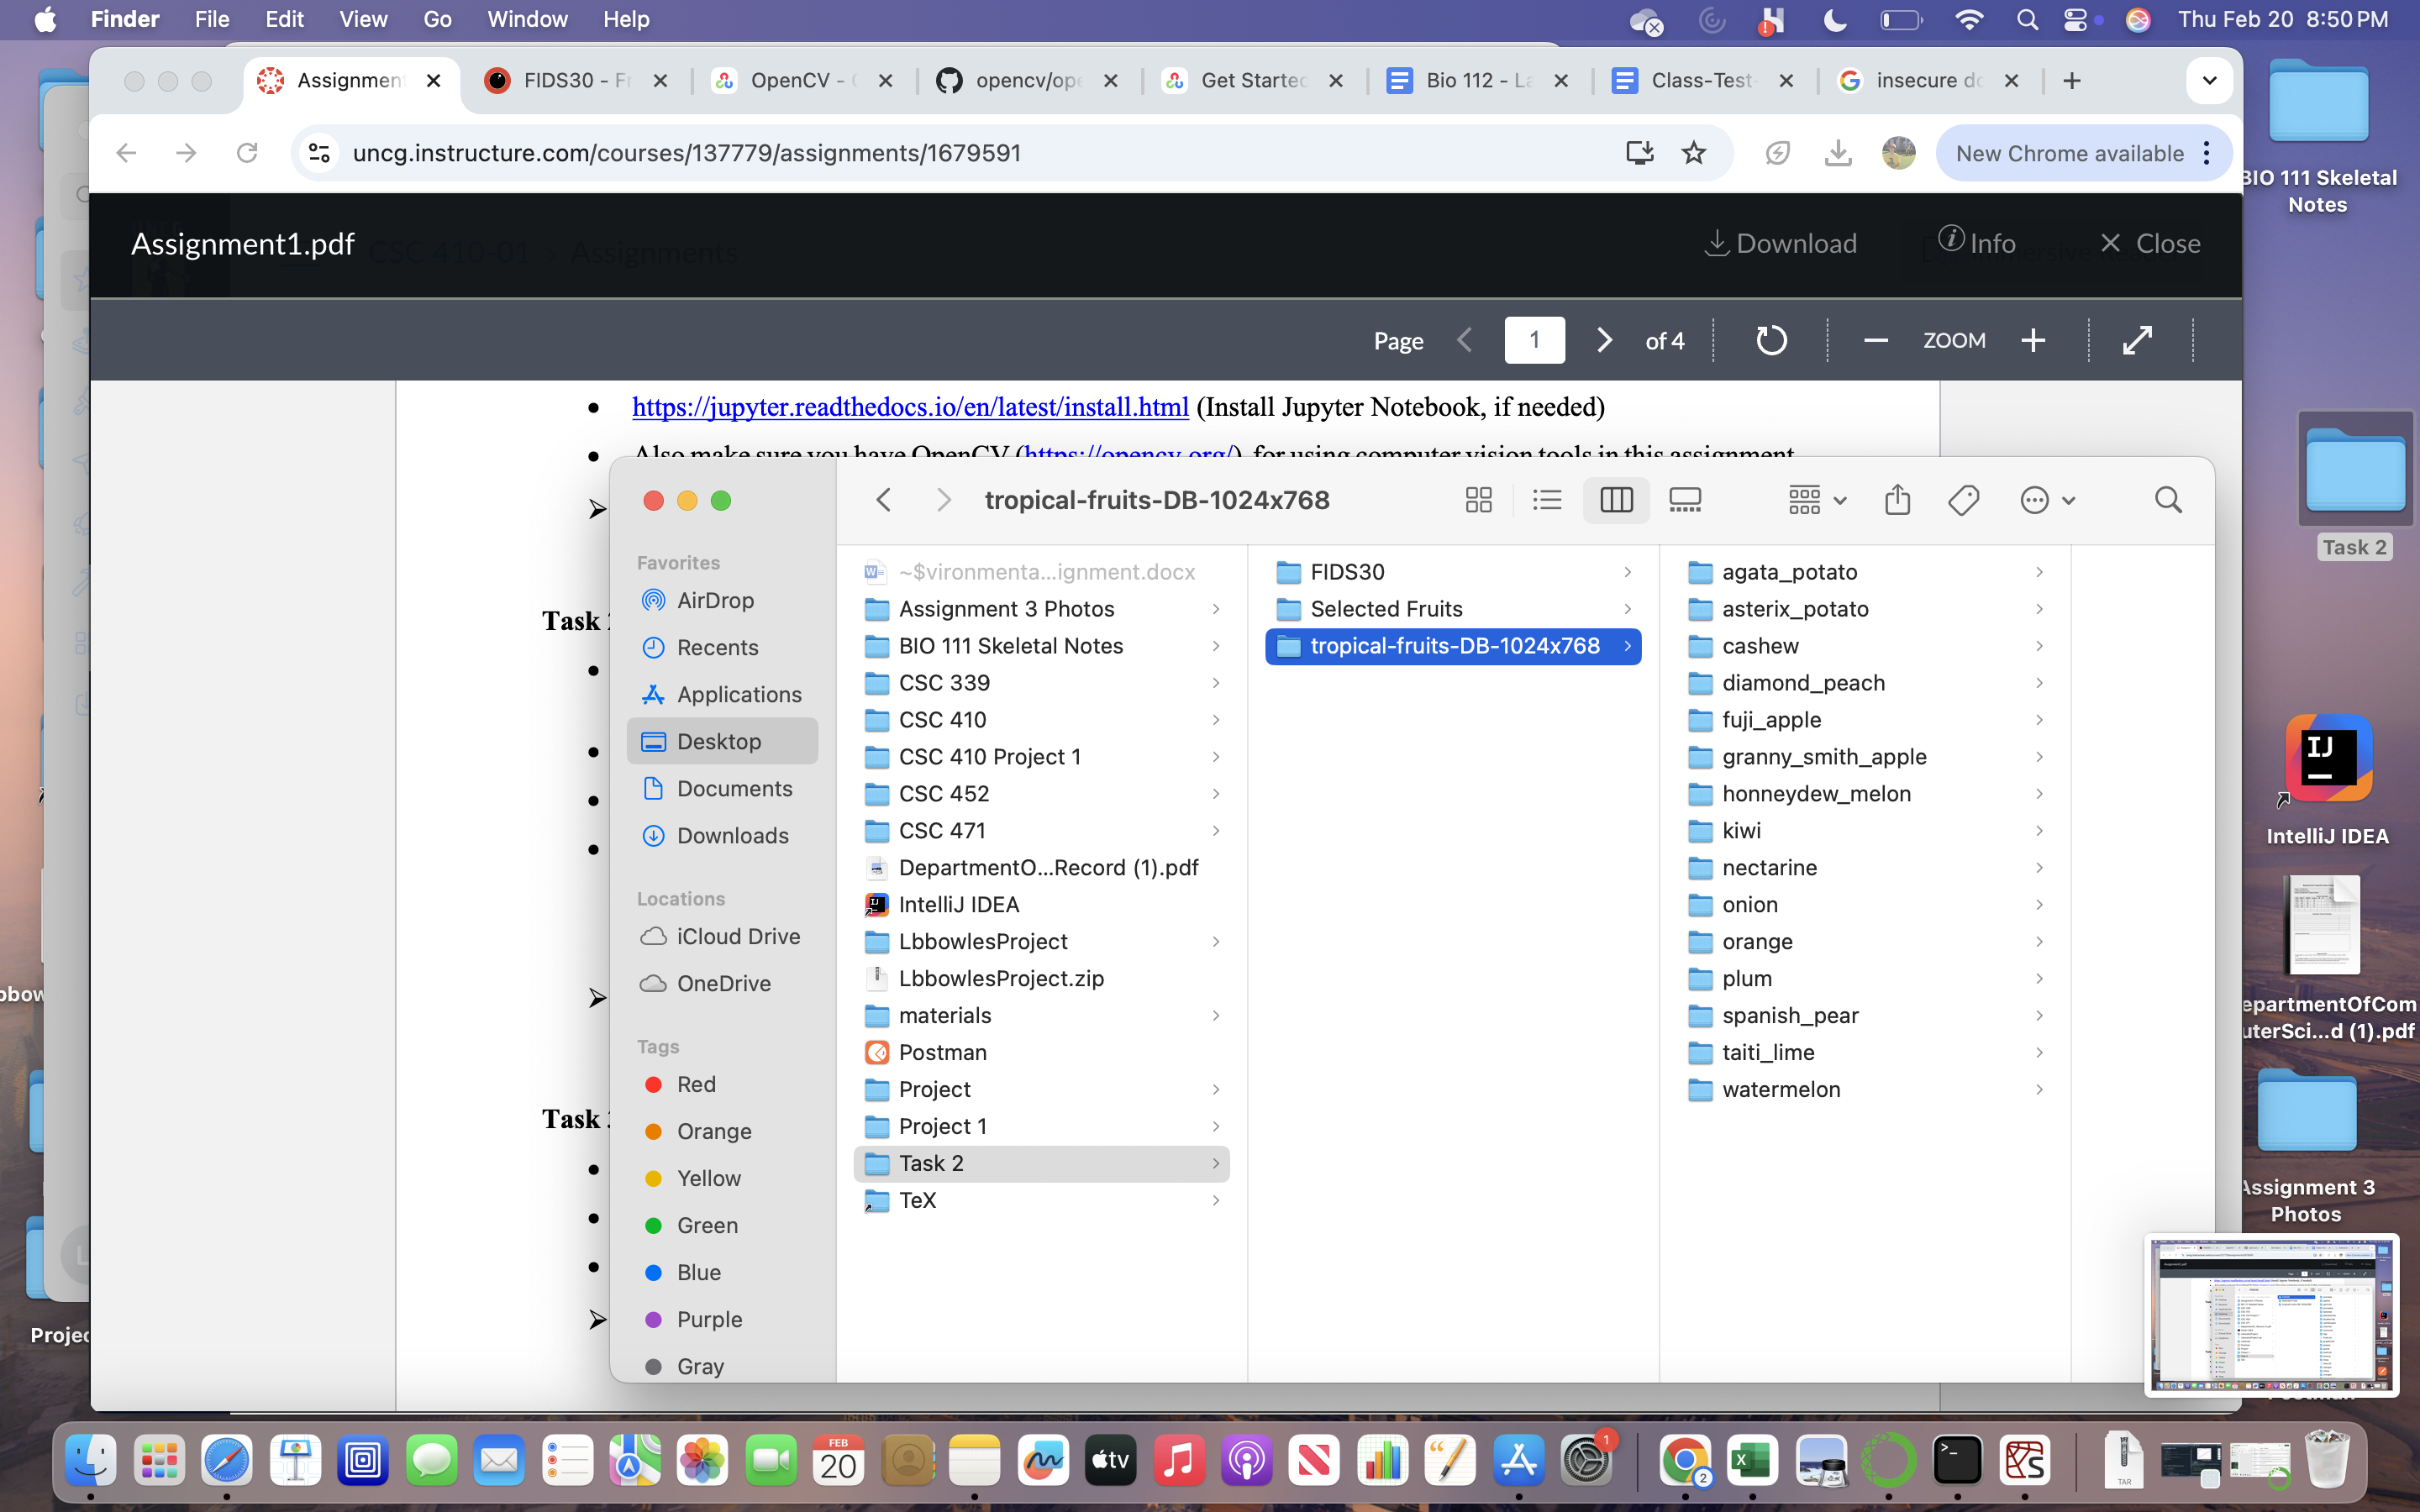
\includegraphics[width=0.5\linewidth]{datafolder2.png}
    \caption{Screenshot of Tropical Fruits folder (not used)}
    \label{fig:screenshot2}
\end{figure}

\begin{thebibliography}{1}
    \bibitem{Skrjanec2013}
    M. Škrjanec and M. Kristan, ``FIDS30 - Fruit Image Data Set,'' 2013. [Online]. Available: \url{https://www.vicos.si/resources/fids30/}. [Accessed: 27-Mar-2025].
\end{thebibliography}

\section{Display Images in Environment and Adjust Color Channels}
This section is focused on images and subsequent manipulation.  The following is the code:

\begin{lstlisting}
folder_path = "/Users/loganbowles/Desktop/Task 2/Selected Fruits"
# Get all image files in the folder that are jpg / jpeg.  Utilizing glob: https://www.geeksforgeeks.org/how-to-use-glob-function-to-find-files-recursively-in-python/#google_vignette
image_files = glob.glob(folder_path + "/*.jpg")

# Loop through each image and display it via plts and cv2
for img_path in image_files:
    img = cv2.imread(img_path)
    img = cv2.cvtColor(img, cv2.COLOR_BGR2RGB)

    # Display images unadulterated and then type shape to the console
    plt.imshow(img)
    plt.title("normal fruit")  
    plt.axis("off")
    plt.show()
    print(f"Image {image_counter}: \nShape: {img.shape}")
    
    #Display different color channels (task 3) -> Code directly from Files in class; just adjusted for my names
    plt.imshow(img[:,:,0], cmap='Blues')
    plt.axis('off')
    plt.show()
    plt.imshow(img[:,:,1], cmap='Greens')
    plt.axis('off')
    plt.show()
    plt.imshow(img[:,:,2], cmap='Reds')
    plt.axis('off')
    plt.show()

    # Convert to grayscale. Also from files
    image_gray = cv2.cvtColor(img, cv2.COLOR_BGR2GRAY)
    
    resized_gray = image_resize(image_gray, height=256)
    plt.imshow(resized_gray, cmap='gray')
    plt.title("gray image")
    plt.axis("on")
    plt.show()
    print(f"New Shape: {resized_gray.shape}")
    
\end{lstlisting}
Explanation: The code is nothing too complicated, and as is visible within its contents, is compliant with Task 10 as I had read ahead while writing it up.  It first designates a folder path, then utilizes glob and a for loop to capture all of the contents within the folder that are jpg/jpeg (as I was having issues when just using jpg for some reason), the for loop, which I essentially grabbed from the class files, plots the images to Anaconda using CV2 and then prints their shape (dimensions).  More class files contained code on how to change the color channel so I just make the for loop use that code to print the different channels and then finally converted it to grayscale.  Now that it has been explained, I will showcase what was returned to console after the code is run.
\begin{lstlisting}
Image 1: 
Shape: (800, 1200, 3)
Image 2: 
Shape: (2223, 2223, 3)
Image 3: 
Shape: (282, 425, 3)
\end{lstlisting}
For the rest of this section, it obviously printed a lot of figures so I am going to place them below as Figures \ref{fig:normal1}-\ref{fig:gray3}, which should conclude this section.

\begin{figure}[H]
    \centering
    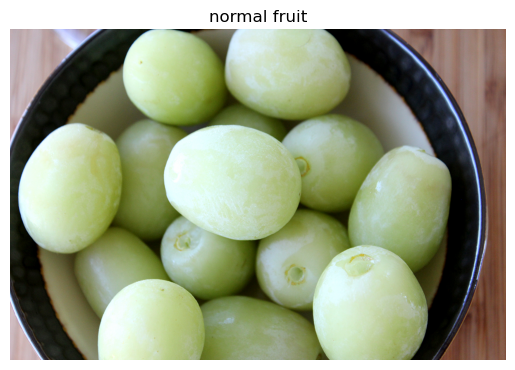
\includegraphics[width=0.5\linewidth]{Task3Output/normalfruit1.png}
    \caption{Output from task 3 - normal}
    \label{fig:normal1}
\end{figure}

\begin{figure}[H]
    \centering
    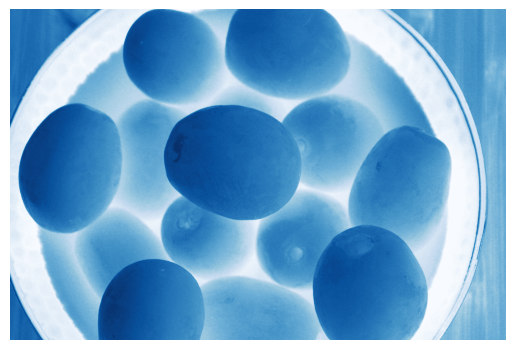
\includegraphics[width=0.5\linewidth]{Task3Output/blue1.png}
    \caption{Output from task 3 - blue channel}
    \label{fig:blue1}
\end{figure}

\begin{figure}[H]
    \centering
    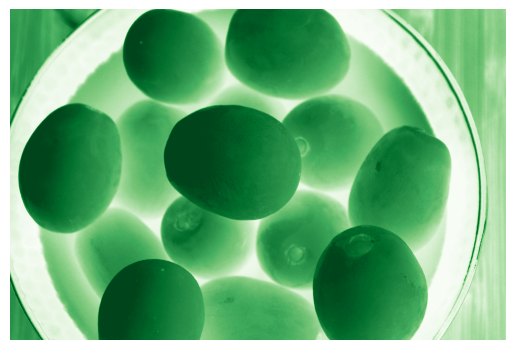
\includegraphics[width=0.5\linewidth]{Task3Output/green1.png}
    \caption{Output from task 3 - green channel}
    \label{fig:green1}
\end{figure}

\begin{figure}[H]
    \centering
    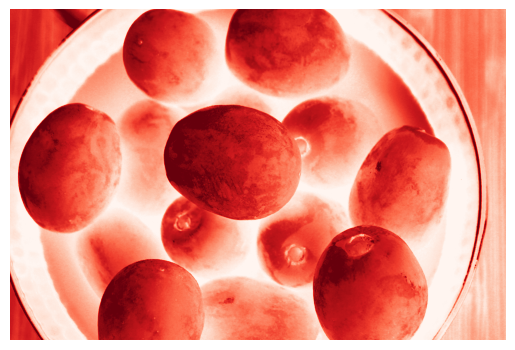
\includegraphics[width=0.5\linewidth]{Task3Output/red1.png}
    \caption{Output from task 3 - red channel}
    \label{fig:red1}
\end{figure}

\begin{figure}[H]
    \centering
    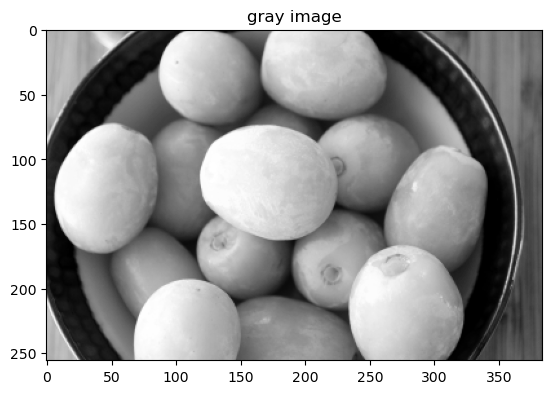
\includegraphics[width=0.5\linewidth]{Task3Output/gray1.png}
    \caption{Output from task 3 - gray channel}
    \label{fig:gray1}
\end{figure}

\begin{figure}[H]
    \centering
    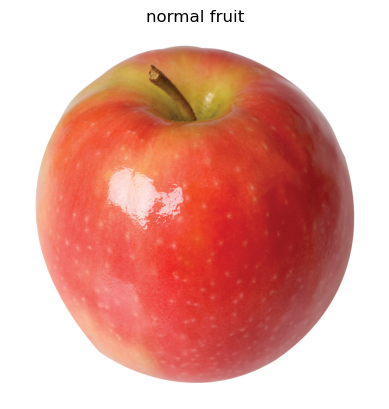
\includegraphics[width=0.5\linewidth]{Task3Output/normalfruit2.png}
    \caption{Output from task 3 - normal}
    \label{fig:normal2}
\end{figure}

\begin{figure}[H]
    \centering
    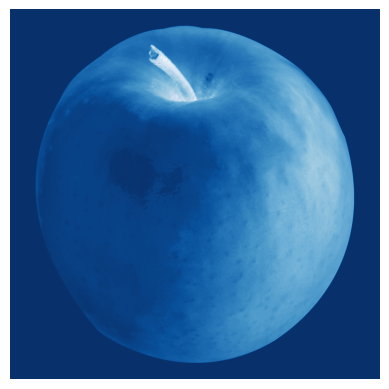
\includegraphics[width=0.5\linewidth]{Task3Output/blue2.png}
    \caption{Output from task 3 - blue channel}
    \label{fig:blue2}
\end{figure}

\begin{figure}[H]
    \centering
    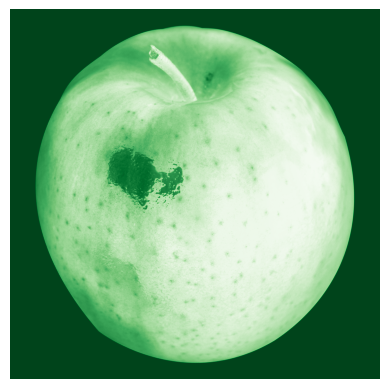
\includegraphics[width=0.5\linewidth]{Task3Output/green2.png}
    \caption{Output from task 3 - green channel}
    \label{fig:green2}
\end{figure}

\begin{figure}[H]
    \centering
    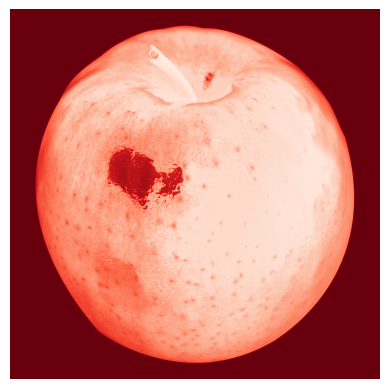
\includegraphics[width=0.5\linewidth]{Task3Output/red2.png}
    \caption{Output from task 3 - red channel}
    \label{fig:red2}
\end{figure}

\begin{figure}[H]
    \centering
    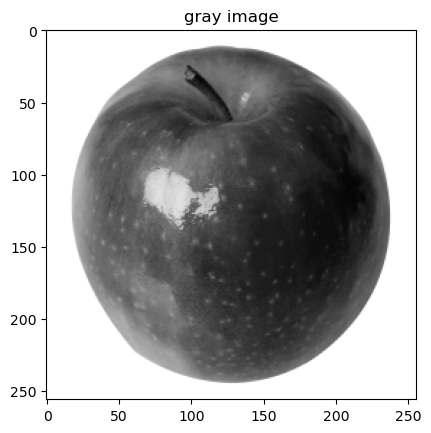
\includegraphics[width=0.5\linewidth]{Task3Output/gray2.png}
    \caption{Output from task 3 - gray channel}
    \label{fig:gray2}
\end{figure}

\begin{figure}[H]
    \centering
    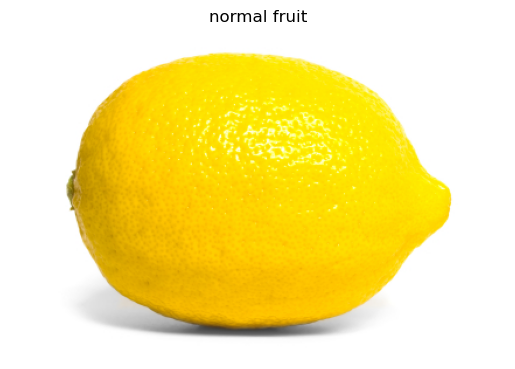
\includegraphics[width=0.5\linewidth]{Task3Output/normalfruit3.png}
    \caption{Output from task 3 - normal}
    \label{fig:normal3}
\end{figure}

\begin{figure}[H]
    \centering
    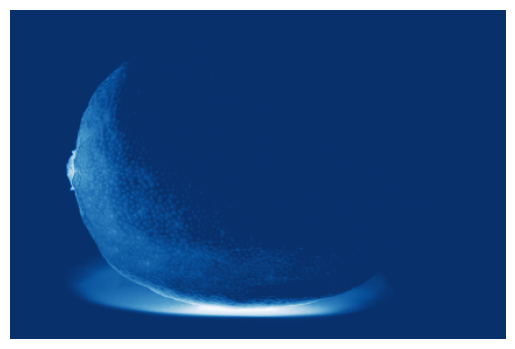
\includegraphics[width=0.5\linewidth]{Task3Output/blue3.png}
    \caption{Output from task 3 - blue channel}
    \label{fig:blue3}
\end{figure}

\begin{figure}[H]
    \centering
    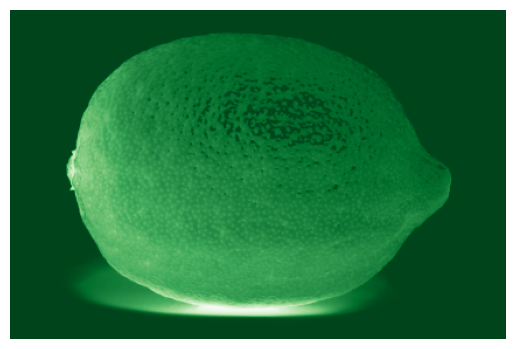
\includegraphics[width=0.5\linewidth]{Task3Output/green3.png}
    \caption{Output from task 3 - green channel}
    \label{fig:green3}
\end{figure}

\begin{figure}[H]
    \centering
    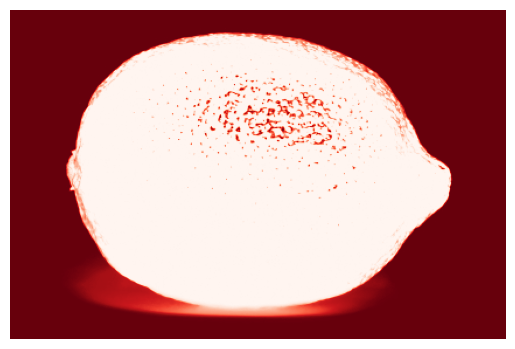
\includegraphics[width=0.5\linewidth]{Task3Output/red3.png}
    \caption{Output from task 3 - red channel}
    \label{fig:red3}
\end{figure}

\begin{figure}[H]
    \centering
    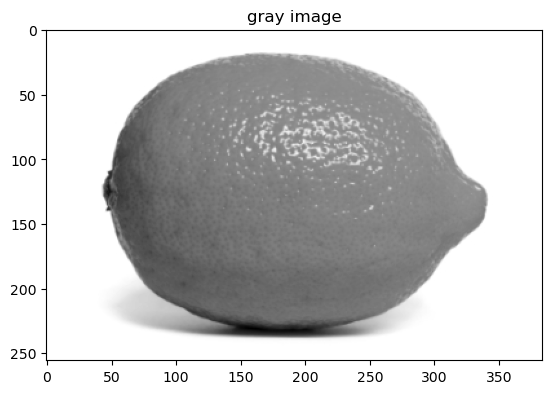
\includegraphics[width=0.5\linewidth]{Task3Output/gray3.png}
    \caption{Output from task 3 - gray channel}
    \label{fig:gray3}
\end{figure}

\section{Reduce Image Dimension}
At first I was truthfully pretty confused about what was meant by keeping the "original aspect ratio" until we discussed it in class.  Once that simple formula was determined, I was able to write the relevant function up without any real issues.  The function is below:
\begin{lstlisting}
# Step 4 function; simple code to find the original dimensions and resize it to meet assignment requirements
def image_resize(image_gray, height=256):
    
    # First ascertain the H x W of the image
    himg, wimg = image_gray.shape
    
    # Formula for aspect ratio and incorporating it to determine the width applicable
    aspect_ratio = wimg / himg
    new_width = int(height * aspect_ratio)
    
    # As per assignment, make sure that it is divisible by 8 (utlize remainder to do so)
    new_width = new_width - (new_width % 8)
    
    # Resize image and return it -> function complete
    resized_gray = cv2.resize(image_gray, (new_width, height), interpolation=cv2.INTER_AREA)
    
    return resized_gray
\end{lstlisting}

After adding the above function and then running the same program again with the only difference being the inclusion of 
\begin{lstlisting}
     resized_gray = image_resize(image_gray, height=256)
    plt.imshow(resized_gray, cmap='gray')
    plt.title("gray image")
    plt.axis("on")
    plt.show()
    print(f"New Shape: {resized_gray.shape}")
\end{lstlisting}
you then get the following returned to the console:
\begin{lstlisting}
    Image 1: 
Shape: (800, 1200, 3)
New Shape: (256, 384)
Image 2: 
Shape: (2223, 2223, 3)
New Shape: (256, 256)
Image 3: 
Shape: (282, 425, 3)
New Shape: (256, 384)
\end{lstlisting}
This confirms that the images were successfully resized and meet the requirements of this task.

\section{Generating Block Feature Vectors - Pooling Effect}
Finally getting into gathering our features and we start with vectorization using the pooling effect.  Utilizing the PDF description, in-class discussion, and the figure at the bottom of Assignment1.pdf - we can finally set ourselves up for feature extraction.  I achieved this effect by creating a new function 'myBlocks' which was mostly from our class files and made slight alterations as needed.  The following is the function:
\begin{lstlisting}
    def myBlocks(img, label):
    
    # Ascertain the height and the width of the image (already resized)
    himg, wimg = img.shape
    
    # Count the number of 8 by 8 blocks that fit in the image exactly
    cellc = (himg // 8) * (wimg // 8)
    
    # Vector storage; intialize all as 0.  64 spots for data and 1 spot for result.
    flatc = np.zeros((cellc, 65), np.uint8)
    
    # Traverse through every block, left to right, then down, repeat until all traversed
    k = 0
    for i in range(0,himg,8):
        for j in range(0,wimg,8):
            
            # Extract an 8x8 block
            crop_tmp1 = img[i:i+8,j:j+8]
            
            # Vectorize / flatten the block
            flatc[k,0:64] = crop_tmp1.flatten()
            # Assign label to end
            flatc[k, 64] = label 
            
            # Move to next row
            k = k + 1
            
    # Return number of 8x8 blocks and flatc
    return cellc, flatc
\end{lstlisting}

I feel it is kind of a waste of time to describe it further than the comments, but in synopsis, we create vector storage in the array flatc where each item is an 8x8 block.  We iterate through the current image and flatten each block into a feature vector and then store it in flatc.  Ultimately, returning the cellc and flatc.  Below this, I am about to put the code that is in the for loop which is actually what is calling this function for every single photo in the folder - but before I do, I wanted to explain that the variable \texttt{'all\_data'} was initialized before the loop with the simple code 
\begin{lstlisting}
    all_data = []
\end{lstlisting}
This will be used for randomization later. Now that the variable has been addressed, the rest of the code is 
\begin{lstlisting}
    # Generate feature vectors and add labels by calling myBlocks function.  Goal is to only extract the array so we ignore the cell count.  feature_vectors will be tbe list of all vectors
    _, feature_vectors = myBlocks(resized_gray, label=image_counter - 1)  
    
    # Convert to an array
    feature_vectors = np.array(feature_vectors)  
    
    # Using a dataframe to create a csv: https://www.geeksforgeeks.org/saving-a-pandas-dataframe-as-a-csv/
    df = pd.DataFrame(feature_vectors, columns=[f"feature_{i}" for i in range(64)] + ["label"])

    # Save to desired location
    csv_path = f"/Users/loganbowles/Desktop/Task 2/feature_vectors_{image_counter-2}.csv"
    df.to_csv(csv_path, index=False)
    
    # Printing the file location just so it is easy to validate
    print(f"Saved: {csv_path}\n")
    
    # Store this iteration to the end of the all_data array to merge after all images have been completed
    all_data.append(df)
\end{lstlisting}
The CSV files will be located within the ZIP folder because it would be a waste of space to show them here (for obvious reasons). Therefore, just know they will not be shown anywhere in this document unless asked by other tasks to do so explicitly.  The final requirement of this task is to merge and randomize the CSV's which I will put the code to below:

\begin{lstlisting}
    # Merge all of the dataframes that are currently in "all_data" into a single dataframe
merged_df = pd.concat(all_data, ignore_index=True)

# Shuffle the dataframe: https://www.geeksforgeeks.org/pandas-how-to-shuffle-a-dataframe-rows/
merged_df = merged_df.sample(frac=1)

# Save merged dataset
merged_csv_path = "/Users/loganbowles/Desktop/Task 2/merged_feature_vectors.csv"
merged_df.to_csv(merged_csv_path, index=False)

# Printing the file location just so it is easy to validate
print(f"Merged dataset saved: {merged_csv_path}")
\end{lstlisting}

Finally, the last thing of note will be the acknowledgment that gets printed to the console as you can see in the above code.  I will put that message here to finish off the section.

\begin{lstlisting}
Image 1: 
Shape: (800, 1200, 3)
New Shape: (256, 384)
Saved: /Users/loganbowles/Desktop/Task 2/feature_vectors_1.csv

Image 2: 
Shape: (2223, 2223, 3)
New Shape: (256, 256)
Saved: /Users/loganbowles/Desktop/Task 2/feature_vectors_2.csv

Image 3: 
Shape: (282, 425, 3)
New Shape: (256, 384)
Saved: /Users/loganbowles/Desktop/Task 2/feature_vectors_3.csv
Merged dataset saved: /Users/loganbowles/Desktop/Task 2/merged_feature_vectors.csv
\end{lstlisting}

\section{Sliding Block Feature Vectors - Convulsion Effect}
As would be expected, this section will be very similar to the last one with the only difference being how the Feature Vectors are assembled - this time using sliding blocks.  This was a pretty hard change for my brain to wrap around, but with the previous function already made, more in-class discussion, and the image in the Assignment PDF I was able to achieve an updated function for sliding with the following code:
\begin{lstlisting}
    def slideBlocks(img, label):
    
    block_size = 8
    slide = 4
    
    # Ascertain the height and the width of the image (already resized)
    himg, wimg = img.shape
    
    # Number of sliding windows that fit horizontally and vertically
    num_cells_vertical = (himg - block_size) // slide + 1
    num_cells_horizontal = (wimg - block_size) // slide + 1
    
    # Total number of sliding windows
    cellc = num_cells_vertical * num_cells_horizontal
    
    
    # Initialize array to store flattened feature vectors, add one for label
    flatc = np.zeros((cellc, block_size * block_size + 1), np.uint8)
    
    
    # Traverse through every block, left to right, then down, repeat until all traversed
    k = 0
    for i in range(0, himg - block_size + 1, slide):
        for j in range(0, wimg - block_size + 1, slide):
            
            # Extract an 8x8 block
            crop_tmp1 = img[i:i+block_size, j:j+block_size]
            
            # Vectorize / flatten the block
            flatc[k, 0:block_size * block_size] = crop_tmp1.flatten()
            # Assign label to end
            flatc[k, block_size * block_size] = label 
            
            # Move to next row
            k = k + 1
            
    # Return number of 8x8 blocks and flatc
    return cellc, flatc
\end{lstlisting}

As aforementioned, a large part of the code is identical, with there being some additional Math that has to be done to achieve the sliding effect.  First thing of note being the 'slide' variable which allows the blocks to move 4 blocks horizontally and vertically allowing for overlapping data unlike the previous function.  We then calculate how many are possibly like we did before and then from that point, the code is pretty much the same.  Just like the last section, I will showcase the code that resides within the for loop and also just like last time, I have created a new array variable this time called \texttt{'all\_data\_sliding'} which does the same thing as the last one and will not appear in the code as it is before the for loop and it is not worth putting the whole for loop for sake of space efficiency:

\begin{lstlisting}
     # Finishing step 6, obviously the same logic, just save them with different file names.
    # Generate feature vectors and add labels again but this time by calling the slideBlocks function.  
    _, feature_vectors = slideBlocks(resized_gray, label=image_counter - 1)  
    
    # Convert to an array
    feature_vectors = np.array(feature_vectors)  
    
    # Using a dataframe to create a csv: https://www.geeksforgeeks.org/saving-a-pandas-dataframe-as-a-csv/
    df = pd.DataFrame(feature_vectors, columns=[f"feature_{i}" for i in range(64)] + ["label"])

    # Save to desired location
    csv_path = f"/Users/loganbowles/Desktop/Task 2/feature_vectors_slide_{image_counter-2}.csv"
    df.to_csv(csv_path, index=False)
    
    # Printing the file location just so it is easy to validate
    print(f"Saved: {csv_path}\n")
    
    # Store this iteration to the end of the all_data array to merge after all images have been completed
    all_data_sliding.append(df)
\end{lstlisting}

The ending is also the same, but for congruency I will show it this time without comments:

\begin{lstlisting}
    # Merge and save sliding window feature vectors, same logic as above.
merged_sliding_df = pd.concat(all_data_sliding, ignore_index=True)
merged_sliding_df = merged_sliding_df.sample(frac=1)  
merged_sliding_csv = "/Users/loganbowles/Desktop/Task 2/merged_feature_vectors_sliding.csv"
merged_sliding_df.to_csv(merged_sliding_csv, index=False)
print(f"Merged sliding dataset saved: {merged_sliding_csv}")
\end{lstlisting}

Finally this confirmation is printed to the console as such:

\begin{lstlisting}
    Image 1: 
Shape: (800, 1200, 3)
New Shape: (256, 384)
Saved: /Users/loganbowles/Desktop/Task 2/feature_vectors_1.csv

Image 2: 
Shape: (2223, 2223, 3)
New Shape: (256, 256)
Saved: /Users/loganbowles/Desktop/Task 2/feature_vectors_2.csv

Image 3: 
Shape: (282, 425, 3)
New Shape: (256, 384)
Saved: /Users/loganbowles/Desktop/Task 2/feature_vectors_3.csv
Merged dataset saved: /Users/loganbowles/Desktop/Task 2/merged_feature_vectors.csv
Merged sliding dataset saved: /Users/loganbowles/Desktop/Task 2/merged_feature_vectors_sliding.csv
\end{lstlisting}

\section{Statistical Descriptors}
I imagine this to be one of the longer sections of this paper as I will have to explain quite a bit, but that being said, the actual goal is not too difficult.  We are tasked to assemble some statistical information about the data we have collected thus far, starting with the number of observations, dimensions of the data, and means of each feature.  This can be achieved a few ways, but I found it most efficient to just create functions that can be called to do it.  Starting off, we have to read in the information about CSV's and we do that as such:
\begin{lstlisting}
    # Read in the csv files to print information about pooling csvs
image0_df = pd.read_csv("/Users/loganbowles/Desktop/Task 2/feature_vectors_0.csv")
image1_df = pd.read_csv("/Users/loganbowles/Desktop/Task 2/feature_vectors_1.csv")
image2_df = pd.read_csv("/Users/loganbowles/Desktop/Task 2/feature_vectors_2.csv")
\end{lstlisting}
Then we can call the function I made to faciliate printing the above "easy to print" information.
\begin{lstlisting}
    def csv_statistics(df, name):
    print(f"\n{name} Stats")
    print(f"Number of observations: {df.shape[0]}")
    print(f"Number of features: {df.shape[1]-1}")
    print("Rest of relevant information\n")
    print(df.describe())
\end{lstlisting}
This code is very simple.  Prints the name so we know what is referring to, then the [0] column as that tells us how many rows (observations) are present, then we can print the features off by printing the columns-1 (to compensate for the label), then finally, we can use the built in feature of .describe() to print other related information such as count, mean, standard deviation, minimum, maximum, etc.  This function obviously works with any dataframe passed to, so it so works with the sliding and non-sliding CSV's allowing for incredibly simple re-utilization.  Below is an example of what is printed to the console:
\begin{lstlisting}
    image01_pooling Stats
Number of observations: 1536
Number of features: 64
Rest of relevant information

         feature_0    feature_1    feature_2  ...   feature_62   feature_63   label
count  1536.000000  1536.000000  1536.000000  ...  1536.000000  1536.000000  1536.0
mean    134.373047   134.735677   134.902344  ...   133.476562   133.921875     1.0
std      71.448208    71.291888    71.335284  ...    71.258968    70.883750     0.0
min       0.000000     0.000000     0.000000  ...     0.000000     0.000000     1.0
25%      79.750000    80.000000    80.000000  ...    81.000000    82.000000     1.0
50%     141.000000   140.000000   141.000000  ...   138.000000   139.000000     1.0
75%     191.000000   190.250000   191.000000  ...   190.000000   190.000000     1.0
max     255.000000   255.000000   254.000000  ...   255.000000   254.000000     1.0
\end{lstlisting}

Now that the numbers have been printed, we can move onto graphing this data.  I decided that it would be the best to utilize Histograms as my graph of choice and just made another very simple function that can be called by any of the CSV's.  These histograms get inspiration from the Histograms in Chapter 3 and therefore are printing information about a specific feature in a very basic histogram - as I feel that it suffices for what it was supposed to achieve.  Here is the function:

\begin{lstlisting}
    # Step 7 code to print histograms as graph of choice.  Used inspiration from Chapter 3 in regards to visual and what it is showing.

def plot_histograms(df, name, feature_idx=32):

    plt.figure()
    plt.hist(df[f"feature_{feature_idx}"], bins=20, color='blue', edgecolor='black')
    plt.title(f"{name} - Feature 32 Distribution")
    plt.xlabel("Feature Value")
    plt.ylabel("Frequency")
    plt.grid(True)
    plt.show()
\end{lstlisting}

here is an example of a line that would call it \texttt{plot\_histograms('image1\_df', "Image02 Pooling")} 
and I will attach the relevant histogram below as figure \ref{fig:histogram}.  I could attach more histograms as it prints one out for every single sliding and pooling CSV but it is kind of repetitive as I made my function only check for feature 32 and this document is already long enough. 

\begin{figure}[H]
    \centering
    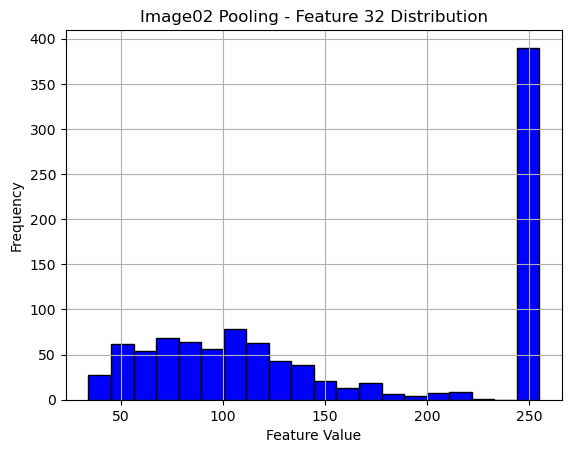
\includegraphics[width=0.5\linewidth]{Task3Output/histogram.png}
    \caption{Histogram plotting data related to feature 32 for the Pooling effect with image02}
    \label{fig:histogram}
\end{figure}

Is the data imbalanced?
Is the data inaccurate or incomplete?
Is the data trivial or big data?
Does the data have a scalability problem?
Is the data high dimensional?
Do I need to standardize the data?
Do I need to normalize the data?
How are the data characteristics affected?

\section{Feature Space Construction}
All of the assignment has built up to this moment, constructing the feature space and thankfully the majority of leg work is behind us as I can follow the Assignment instructions to pretty easily construct the feature spaces I am being told to create with the code below:

\begin{lstlisting}
    # Merge the csvs by stacking rows
image01_df = pd.concat([image0_df, image1_df], ignore_index=True)

# Shuffle the dataset (row order only)
image01_df = image01_df.sample(frac=1)  

# Save as image01.csv
image01_csv_path = "/Users/loganbowles/Desktop/Task 2/image01.csv"
image01_df.to_csv(image01_csv_path, index=False)

# Printing the file location just so it is easy to validate
print(f"Feature space for image01.csv saved: {image01_csv_path}")

# Move to next part of Step 8, attaining features from all three images.

# Merge image0, image1, and image2
image012_df = pd.concat([image0_df, image1_df, image2_df], ignore_index=True)

# Shuffle the dataset
image012_df = image012_df.sample(frac=1)

# Save as image012.csv
image012_csv_path = "/Users/loganbowles/Desktop/Task 2/image012.csv"
image012_df.to_csv(image012_csv_path, index=False)

print(f"Feature space for image012.csv saved at: {image012_csv_path}")
\end{lstlisting}
As can be seen above, this is not really that involved and the comments iterate my thought process throughout.  That being said, I can finally see the below message in my console and of course the CSV files are being saved where they are supposed to be saved.
\begin{lstlisting}
Feature space for image01.csv saved: /Users/loganbowles/Desktop/Task 2/image01.csv
Feature space for image012.csv saved at: /Users/loganbowles/Desktop/Task 2/image012.csv
\end{lstlisting}

\section{Display Multi-Feature Subspaces}
Now that we have our 2 and 3 dimensional subspaces created, it makes sense for us to actually showcase them via a plot - we can do so by loading it up with 
\texttt{df = pd.read\_csv("\_Users\_loganbowles\_Desktop\_Task\ 2\_image01.csv")}
then sub-sequentially run the following code to actually generate our graph based on our features (I just chose 1 and 2)

\section{Update Code to Work With More Images}
I have already addressed this and actually begun my code with resolving this issue via glob. First visualization of this is in Section 3 where I put the code I have made.  This section has been completed.

\section{Effects of Block Size on Dimensionality}
This section is a little bit different, more so focused on the theory aspect of Machine Learning, in this instance: how would changing the block size affect the dimensionality of the feature space?  The answer is actually pretty obvious - the smaller the blocks being harvested, means the more features can be extracted, therefore making it higher dimensionality and having more features in the feature space.  There are pro's and con's to adding more features, pro's including more nuanced analysis and possibly easier detection of classes with the con's being more complexity/possible overfitting. 

\section{Assignment 2 - Part 1: Extending Assignment 1}
As Assignment 2 is upon us, we are first tasked with a few different precursors - with the first interesting one being to divide the datasets into 80:20 for training and testing respectively.  This step really was not bad considering that the class file 'class-code-ridge-reg.txt' shows us directly how to split the data to accomplish such a task and then we just save it the same way that we had been doing with our files beforehand.  Since this is the case, I will not reproduce the code here, I write this after the fact, but do not even recall making any changes and saved it the exact same way so doing so would be kind of redundant. \\
Now that the simplest of the tasks have been completed, we then have to determine if the training and testing sets follow the same distribution which can be done by determining the shape, mean values, and variance.  To achieve this, I knew immediately we could utilize .mean(), .var(), and .shape() to print the information to the console.  After we put in the fairly simple code to do this, (which I will showcase a bit here):
\begin{lstlisting}
# Compute mean and variance
train_mean_1, train_var_1 = X_train[feature_1].mean(), X_train[feature_1].var()
test_mean_1, test_var_1 = X_test[feature_1].mean(), X_test[feature_1].var()

train_mean_2, train_var_2 = X_train[feature_2].mean(), X_train[feature_2].var()
test_mean_2, test_var_2 = X_test[feature_2].mean(), X_test[feature_2].var()

# Get shape of the data
train_shape_1 = X_train[feature_1].shape
test_shape_1 = X_test[feature_1].shape

train_shape_2 = X_train[feature_2].shape
test_shape_2 = X_test[feature_2].shape
\end{lstlisting}

, we get the below section returned to the console.  The only thing I want to put as a note, is that when I was trying to attain the mean and var, I actually was getting a persistent error: 'Could not convert string '{x}' to numeric'.  I then plugged in \texttt{print(X\_train.dtypes)}
and it was returning an object. I then utilized \texttt{https\_colon\_pandas.pydata.org\_docs\_\\reference\_api\_pandas.to\_numeric.html} to resolve this issue with \texttt{pd.to\_numeric} on X\_train and X\_test which allowed for everything to be ascertained error free. Aside from that little 10 minute adventure, things went easily and this was returned to the console:


\begin{lstlisting}
Feature space for image01.csv saved: /Users/loganbowles/Desktop/Task 2/image01.csv
Feature space for image012.csv saved at: /Users/loganbowles/Desktop/Task 2/image012.csv
Training features saved to /Users/loganbowles/Desktop/Task 2/X_train.csv
Training labels saved to /Users/loganbowles/Desktop/Task 2/Y_train.csv
Test features saved to /Users/loganbowles/Desktop/Task 2/X_test.csv
Test labels saved to /Users/loganbowles/Desktop/Task 2/Y_test.csv

Feature 0:
  Train Mean=145.13, Train Var=5751.75, Train Shape=(2048,)
  Test Mean=141.72, Test Var=6330.81, Test Shape=(512,)
Feature 1:
  Train Mean=145.09, Train Var=5731.08, Train Shape=(2048,)
  Test Mean=143.03, Test Var=6308.39, Test Shape=(512,)
\end{lstlisting}
Along with our Figures which I will attach below this section, it is very evident that they have the same distribution, although all of the statistics have very slight numerical deviations, it is an amount that would be deemed safely negligible. \\
For the last part of Task 1, we are tasked to produce Scatterplots for each category of the Training and Testing datasets.  Now this is not the first time that we had to create Scatterplots as we needed to in the first Assignment so some base knowledge was still applicable.  All we had to do was create another plot with 2 subplots - one for training data and the other for testing.  Code for this is of course is within the Python file which has been updated for this submission.  I will try my best to keep straight code usage low for this report as I can see that was written in the directions!  Below are the figures that were generated for this step.

\begin{figure}[H]
    \centering
    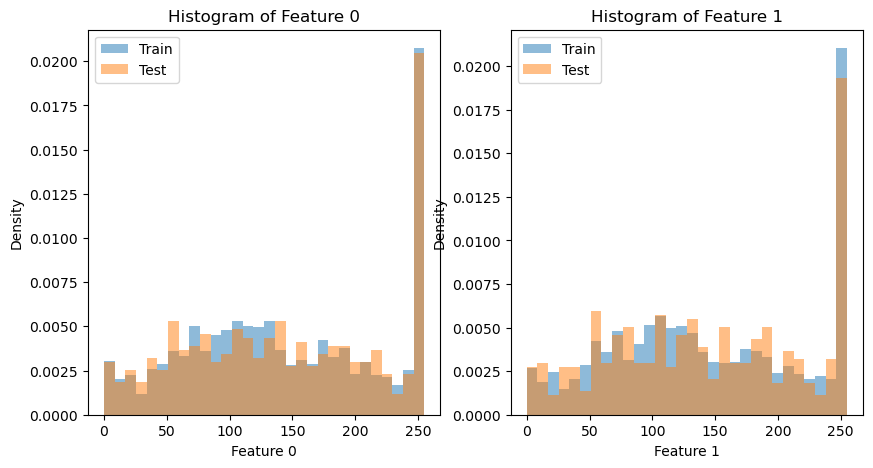
\includegraphics[width=0.5\linewidth]{Part11.png}
    \caption{Histogram plotting distribution}
    \label{fig:histogram1}
\end{figure}

\begin{figure}[H]
    \centering
    \includegraphics[width=0.5\linewidth]{Part12.png}
    \caption{Scatterplot for comparison of Training and Testing.}
    \label{fig:histogram1}
\end{figure}

\section{Regression Based Model}

Task 2 is to introduce a regression-based model in the form of either lasso or elastic-net regression as a two-class classifier.  We then are supposed to form confusion matrices using the responses for the predicted and actual labels and then subsequently save them.  To be fully transparent, I know that the entire point of the first task was to call upon data domains that we just saved (80/20), but throughout this entire task I had a hard time with that so ultimately just reverted to the normal pd.read… route and just copied what was done from the task above into this section.  Luckily for all us students, most of the code I had to use for implementation of Lasso was provided within the class file: "class-code-lasso-reg.txt".  Some of the small tweaks that I made include using 'label' instead of nn for when creating X and y because I was getting an error: could not convert string to float: \texttt{feature\_0} so just .dropping label for X was infinitely easier than trying to troubleshoot anything further.  The other notable change that I made was increasing the max iterations to 10000 - I did this as I received an error in my console intermittently that convergence was not being reached and to resolve that I could simply raise iterations so I did and have stopped having issues.  The Math was already provided in Class Files so very little issues there besides occasional errors about division, so I made it an if statement to resolve that.  Although I will say and you will see from the console output, it is definitely wrong - but I am just using what was provided. \\ When it comes to the Confusion Matrix, I followed lead of the aforementioned class file and actually saved it by turning it into a DF so that I could save it as csv.  Below will be what is printed to console post Task 2.

\begin{lstlisting}
    Lasso: 

Our_Accuracy_Score: 1.0
Our_Precision_Score: 0
Our_Sensitivity_Score: 0
Our_Specificity_Score: 1.0 

Fixed Accuracy Score: 1.0
Fixed Precision Score: 0
Fixed Sensitivity Score: 0
Fixed Specificity Score: 1.0 

BuiltIn_Accuracy: 0.681640625
BuiltIn_Precision: 0.6698564593301436
BuiltIn_Sensitivity (recall): 0.9180327868852459 

   Actual  Predicted
0       1        1.0
1       2        1.0
2       2        1.0
3       1        1.0
4       1        1.0 

Test Reults for test_results.csv saved at: /Users/loganbowles/Desktop/Task 2/test_results.csv

Confusion Matrix:
           Predicted 0  Predicted 1
Actual 0          280           25
Actual 1          138           69 

Confusion matrix saved at: /Users/loganbowles/Desktop/Task 2/confusion_matrix.csv 
\end{lstlisting}

\section{Random Forest}
The goal of Task 3 for Assignment 2 was to utilize Deep Learning or Random Forest (Which I chose) to train for our 2 and 3 class csvs (image01 and image012 for my project.  To utilize this, I followed the path in the instructions for the assignment which led me to: \texttt{https://scikit-learn.org/stable/modules/\\generated/sklearn.ensemble.RandomForest\\Classifier.html}
.  As with all their website, it was very extensively documented and had examples making this somewhat complex topic only take a few lines of code with the package. Specifically, I started off the section of code the same way as the others, pulling in the CSV I am working with (starting with image01 for two classes), then splitting for train/split which while reading, I learned that SciKit also has a function for that \texttt{X\_train, X\_test, y\_train, y\_test = train\_test\_split(X, y, test\_size=0.2)}
 which with that little line of code accomplishes what took multiple in previous sections.  We then can '.fit' (again, utilization of their website basically made this hand-holding) to then finally predict and see the results.  Finally we then save it.  \\ To suffice for Task 4, I decided to read into \texttt{classification\_report} which yet again, is supplied by SciKit.  This shows us the data that is relevant for our accuracy in regard to prediction with 20 characters of code written, super helpful stuff.  \\ Lastly, I had to do this same thing for 3 classes but to achieve this, you literally can copy the code that was just written and replace the csv with our csv that contains 3 classes (image012) then just save our files to a different file path of course.  That concludes Task 3.  Below is the console after running task 3.
\begin{lstlisting}

    ###############
Assignment 2 - Task 3

Random Forest (2-class) 
               precision    recall  f1-score   support

           1       0.86      0.93      0.90       316
           2       0.87      0.77      0.82       196

    accuracy                           0.87       512
   macro avg       0.87      0.85      0.86       512
weighted avg       0.87      0.87      0.87       512

Random Forest (3-class) 
               precision    recall  f1-score   support

           1       0.85      0.89      0.87       305
           2       0.79      0.42      0.54       224
           3       0.72      0.95      0.82       291

    accuracy                           0.78       820
   macro avg       0.79      0.75      0.74       820
weighted avg       0.79      0.78      0.76       820

\end{lstlisting}

\section{Evaluation of Learning Models}
When it comes to measuring performance of the models, I actually took care of these aspects while going through the previous tasks, in the forms of the equations in task 2 (which are shown in the console text) and the same in Task 3 with utilization of the classification\_report.  Therefore making observations is easy to do. \\ I am still working on this project as the days go and wanted to have something worthy of a submission, that being said still have not yet added the "qualitative" bits throughout assignment 2.

\section{Scalable Machine Learning}
Finally we conclude this assignment and do with the ever-daunting task of allowing for scalability.  In this instance we have a few things to quickly go over, firstly - I am very thankful that we were provided most of what was needed to achieve this in the file 'class-code-pca.txt'.  That being said, for my implementation of this, I chose to standardize and then implement PCA.  Now while PCA as we have discussed both in class - and within the confines of the textbook, it is a great tool for large machine learning environments and programs.  Here, it is much less effective.  In all of the testing that I did post implementation, the accuracy in predictability is almost always the same for 2 class identification at least.  Some exceptions for a little more accurate and more exceptions for a little less accurate, in synopsis, it is non-consequential.  Below I will put what is printed to the console.


\begin{lstlisting}

###############
Assignment 3

oob error 
 {0.15087890625} 


Confusion Matrix:
           Predicted 0  Predicted 1
Actual 0          283           36
Actual 1          114           79 

Confusion matrix saved at: /Users/loganbowles/Desktop/Task 2/confusion_matrix.csv 

\end{lstlisting}

For my assignment I only implemented three class identification as I didn't really have time due to other commitments + hoping it would be extended like the predecessors.  That being said, I am almost positive we would get another negligible result if we attempted with three classes.


\bibliographystyle{IEEEtran}

\end{document}
